%-------------------------------------------------------%
%                        第1章内容
%-------------------------------------------------------%
\chapter{基本结构及主要内容}\label{第1章}

\section{基本结构}

学位论文包括前置部分、正文部分和结尾部分共三大部分,各部分组成及顺序如图\ref{fig:学位论文基本结构}所示。

\begin{figure}[h]
    \centering
    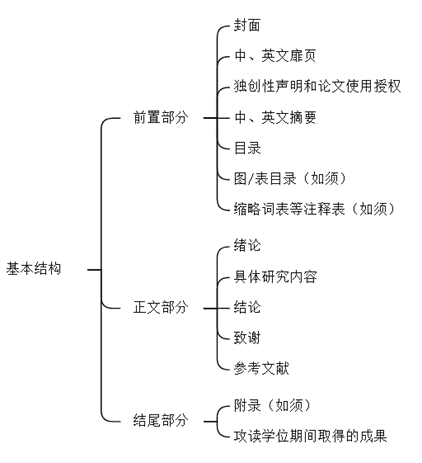
\includegraphics[width=0.7\linewidth]{figures/figure1.png}
    \caption{学位论文基本结构}
    \label{fig:学位论文基本结构}
\end{figure}

\section{前置部分}

\subsection{封面}

不同学位类别对应不同封面。其中,博士学位封面分为精装本、简装本,精装本为绿色漆布材质,烫金字体;硕士学位只有简装本。

论文题目是论文的总纲,是反映论文中重要特定内容的恰当、简明的词语的逻辑组合。题名用词须考虑有助于选定关键词和编制题录、文摘等二次文献所需的使用信息,力求简短,\textbf{避免使用不常用的缩略词、首字母缩写字、字符、代号、公式等,一般不宜超过25字}。

如题名内容层次很多,难以简化时,可采用题名和副题名相结合的方法,副题名起补充、阐明题名的作用。中文的题名与副题名之间用破折号相连,英文则用冒号相连。题名和副题名在整篇学位论文中的不同地方出现时,应保持一致。

指导教师:以研究生管理信息系统登记的责任导师为准,且\textbf{只能填写一名指导教师}。

\subsection{扉页}

学科专业:参照研究生管理信息系统登记的学科专业,以国务院学位委员会批准的学科目录为准。其中,学术学位研究生:按学科目录一级学科培养的,填一级学科;按学校自主设置二级学科培养的,填所属一级学科;按学科目录二级学科培养的,填二级学科。

指导教师:以研究生管理信息系统登记的责任导师为准,若还有其他导师联合指导,可一起填写在扉页,中间用顿号隔开(指导教师最多填2位)。

\textbf{涉密学位论文},按学校相关规定,还须在封面右上角按“密级$\bigstar$保密期限”格式标注,例如“秘密$\bigstar$10年”。

\subsection{独创性声明和论文使用授权}

内容、样式及填写说明见本文档开头部分。除提交盲审的学位论文外,导师及研究生本人须在独创性声明和论文使用授权相应位置签字。

\subsection{摘要}

摘要是学位论文内容不加注释和评论的简短陈述。摘要应具有独立性和自含性,是一篇简短但意义完整的文章,内容应包括研究目的、内容、方法、结果和结论等,\textbf{重点是结果、结论}。

摘要的内容要完整、客观、准确,应做到不遗漏、不拔高、不添加,按层次逐段简要写出。摘要在叙述研究内容、研究方法和主要结论时,除作者的价值和经验判断可以使用第一人称外,一般使用第三人称,采用“分析了……原因”“研究了……”“对……进行了探讨”“给出了……结论”等记述方法进行描述。避免主观性的评价意见,避免对背景、目的、意义、概念和一般性(常识性)理论叙述过多。

摘要需采用规范的名词术语(包括地名、机构名和人名)。对个别新术语或无中文译文的术语,可用外文或在中文译文后加括号注明外文。摘要中应尽量避免使用图、表、化学结构式、非公知公用的符号与术语,不标注引用文献编号。

硕士论文中文摘要\textbf{一般不超过800字,且篇幅控制在1页以内};博士论文中文摘要\textbf{一般不超过1500字,篇幅控制在2页以内}。英文摘要另起一页书写,标题ABSTRACT全部大写,内容与中文摘要一致,翻译准确,博士论文译为“Dissertation”,硕士论文译为“Thesis”。

\subsection{关键词}

关键词是用以表示全文主题内容信息的单词或术语,一般为3~8个。关键词应体现论文特色,具有语义性,在论文中有明确的出处,不应使用太泛指的词,例如“方法”、“理论”、“分析”等。

应尽量采用《汉语主题词表》或各专业主题词提供的规范词。与摘要正文之间空一行顶格书写,用\textcolor{red}{逗号}隔开。若关键词超过一行,换行后应悬挂缩进对齐。英文关键词应与中文关键词对应,每个单词首字母大写。

\subsection{目录}

目录是论文的提纲。\textbf{目录内容从“第1章”开始}至论文最后一页,包含论文正文部分的全部章、节、条三级标题及其起始页码,排在序言或前言之后,另起页。

\subsection{图/表目录}

如果论文中使用了大量的图片或表格,可分别列出索引清单置于目录之后。

图的清单应有序号、图题和页码,表的清单应有序号、标题和页码,样式见本文档图目录。

\subsection{注释表}

如果论文中使用了大量的符号、标志、缩略词、计量单位、自定义名词和术语等,应编写成注释表汇集表置于目录之后。若上述符号使用数量不多,可以不设此部分,但必须在论文中初次出现是加以说明。

符号、缩略词等注释表样式见本文档主要符号表、缩略词表。

\section{正文部分}

正文部分是学位论文的主题和核心部分,一般从绪论开始,包括具体研究内容、结论、参考文献等,应层次分明、逻辑性强。

\subsection{绪论}

绪论(第1章)应简要阐明论文的选题,选题背景及意义,国内外相关研究成果与进展述评,存在的不足或有待进一步研究的问题,本论文所要解决的科学与技术问题、所运用的主要理论和方法、基本思路和论文结构等。

绪论要注意对论文所引用的国内外文献进行准确标注。

\subsection{具体研究内容}

具体研究内容是论文的主要部分,根据学科专业特点和选题情况,可以有不同的写作方式,但应遵循本学科通行的学术规范,必须实事求是,客观真切,准确完备,合乎逻辑,层次分明,重点突出,文字简练、通顺。

学位论文应围绕一个主题,针对某学科领域中的一个具体问题展开深入、系统的研究,并得出有价值的研究结论。论文各章之间应该前后关联,构成一个有机整体。论文给出的数据必须真实可靠,推理正确,结论明确,无概念性和科学性错误。对于科学实验、计算机仿真的条件、实验过程、仿真过程等需加以叙述,然后对结果进行分析及理论提升,避免直接给出结果、曲线和结论。引用他人研究成果或采用他人成果时,应注明出处,不得将其与本人提出的理论分析混淆在一起。

论文各章末尾应有“本章小结”,实验方法或材料等章节可不写“本章小结”。各章小结是对各章研究内容、方法与成果的简洁准确的总结与概括,也是论文最后结论的依据。

\subsection{结论}

结论(最后1章)是论文总体的、最终的结论,并不是各章小结的简单重复,应精炼、准确、完整。结论应包括论文的核心观点,重点阐述论文的创造性工作和创新性成果,及其在本领域内的地位、作用和意义,说明论文研究工作的局限或有待进一步研究和探讨的问题,提出未来工作的设想或建议。

\subsection{致谢}

致谢对象包括资助研究工作的基金、组织或个人,协助完成研究工作的组织或个人,在研究工作中提出重要建议或提供重要帮助的组织或个人以及提供转载和引用权的资料、图片、文献、研究思想和设想的所有者等,\textbf{一般不超过800字}。

\subsection{参考文献}

参考文献应置于正文后,并另起页。

学位论文的撰写应本着严谨求实的科学态度,所有被引用文献均要列入参考文献中,必须按文中出现的顺序标注,但同一篇文献只用一个序号。

尽量引用原始文献。当不能引用原始文献时,要将二次引用文献、原始文献同时标注。\textcolor{red}{博士学位论文的参考文献一般不少于100篇,学术型硕士学位论文的参考文献一般不少于50篇,专业硕士学位论文的参考文献一般不少于30篇,其中外文文献一般不少于总数的1/2}。参考文献中近五年的文献数一般应不少于总数的1/3,并应有近两年的参考文献和一定数量的学位论文或专业名著。

产品说明书、未公开发表的研究报告(著名的内部报告如PB、AD报告及著名大公司的企业技术报告等除外)以及其它无法通过公开途径获得的文献资料通常不宜作为参考文献引用。

引用网上参考文献时,应注明该文献的准确网页地址,网上参考文献和各类标准不包含在上述规定的文献数量之内。\textbf{本人在攻读学位期间发表的学术论文不应列入参考文献中},具体格式要求见\ref{sec2.9}节。

\section{结尾部分}

\subsection{附录}

附录是作为论文主体的补充项目(非必须),主要包括正文内不便列出的冗长公式推导、某些重要的原始数据、计算程序及说明等。文中的附录A、B、C仅供做参考,不出现在正文中。

\subsection{攻读学位期间取得的研究成果}

在攻读博士(硕士)学位期间取得的与论文内容相关的研究成果,例如:发表和已录用的学术论文、专著/译著、参与的科研项目、专利、作品、科研获奖等。与学位论文无关的学术论文不宜在此列出,具体格式要求见\ref{sec2.10}节。

\section{各部分标题英文翻译}

用英文撰写的学位论文,内容、格式要求与中文学位论文一致。各部分标题中英文翻译对照如\ref{tab1-1}所示。

\begin{table}[!ht]
\centering
\caption{学位论文各部分标题中英文翻译对照表}
\label{tab1-1}
\begin{tabularx}{\textwidth}{ 
>{\centering\arraybackslash}X 
>{\centering\arraybackslash}X
}
\toprule
中文 & 英文 \\
\midrule
摘要 & ABSTRACT \\
目录 & Contents \\
图目录 & Figures \\
表目录 & Tables \\
主要符号表 & Symbols \\
缩略词表 & Acronyms \\
参考文献 & References \\
致谢 & Acknowledgements \\
附录(附录A,附录B......) & Appendix (Appendix A, Appendix B...) \\
\bottomrule
\end{tabularx}
\end{table}

\section{本章小节}

本章主要对学位论文的基本结构和主要内容进行了详细说明。